\sectionthree{Linear homogeneous recurrence relations of degree 2: complex case}
\begin{python0}
from solutions import *; clear() 
\end{python0}

Recall that following facts derived for the homogeneous recurrence
relation of degree 2
: Our recurrence relation is this:
\[
a_n = c_1 a_{n-1} + c_2 a_{n-2}, \,\,\,\,\, (n \geq 2)
\]
and the rational function for $a(x) = \sum_{n=0}^\infty a_n x^n$ is
\[
\frac
{a_0 + (a_1 - c_1 a_0) x}
{1 - (c_1 x + c_2 x^2)}
\]
The denominator of the rational function is
\begin{align*}
1 - (c_1 x + c_2 x^2)
&= -c_2 \biggl( x^2 + \frac{c_1}{c_2} x - \frac{1}{c_2} \biggr)
\end{align*}
The roots of
\[
x^2 + \frac{c_1}{c_2} x - \frac{1}{c_2}
\]
are
\[
x
=
\frac{-c_1 \pm \sqrt{c_1^2 + 4c_2}}{2c_2}
\]
Therefore $a(x)$ looks like this:
\begin{align*}
a(x) 
&=
\frac {a_0 + (a_1 - c_1 a_0) x} {-c_2} \cdot
\frac{1}{x^2 + \frac{c_1}{c_2} x - \frac{1}{c_2}} \\
&= (A + Bx) \frac{1}{(x-C)(x-D)}
\end{align*}
where
\[
A = -\frac{a_0}{c_2}, \,\,\,\,\, B = -\frac{a_1 - c_1 a_0}{c_2}
\] 
and for $C$ and $D$ are distinct roots of the
denominator of the rational function of $a(x)$:
\[
C = \frac{-c_1 - \sqrt{c_1^2 + 4c_2}}{2c_2},
D = \frac{-c_1 - \sqrt{c_1^2 + 4c_2}}{2c_2}
\]

Note that it's possible to have complex roots.

Let's pause here to try an example where the roots are complex.
Consider the case where
\[
a_n 
= 
\begin{cases}
1 & \text{ if } n = 0, 1 \\
-a_{n-2} & \text{ if } n \geq 2
\end{cases}
\]

In this case
\[
a(x) 
= \frac{1 + x}{1 + x^2} 
= \frac{1 + x}{(x - i)(x + i)}
\]
Now 
\[
\frac{1}{(x-i)(x+i)}
=
\frac{1}{2i} 
\biggl(
\frac{1}{x - i}
-
\frac{1}{x + i}
\biggr)
\]
(make sure you derive this) and hence

\begin{align*}
a(x) 
&= \frac{1 + x}{1 + x^2} = \frac{1 + x}{(x - i)(x + i)} =(1+x) \cdot
\frac{1}{2i} 
\biggl(
\frac{1}{x - i}
-
\frac{1}{x + i}
\biggr) \\
&= (1+x) \cdot \frac{1}{2i}
\biggl(
-\frac{1}{i - x}
-
\frac{1}{i - (-x)}
\biggr) \\
&= (1+x) \cdot \frac{1}{2i}
\biggl(
-\frac{1}{i}\frac{1}{1 - x/i}
-
\frac{1}{i}\frac{1}{1 - (-x)/i}
\biggr) \\
&= (1+x) \cdot \frac{1}{2i} \cdot \frac{-1}{i}
\biggl(
\sum_{n=0}^\infty \biggl( \frac{x}{i} \biggr)^n
+
\sum_{n=0}^\infty \biggl( \frac{-x}{i} \biggr)^n
\biggr) \\
&= (1+x) \cdot \frac{1}{2}
\sum_{n=0}^\infty 
\biggl(
\biggl(
\frac{1}{i} 
\biggr)^n
+
\biggl(
\frac{-1}{i} 
\biggr)^n
\biggr) 
x^n \\
&= (1+x) \cdot \frac{1}{2}
\sum_{n=0}^\infty 
\biggl(
\frac{1 + (-1)^n}{i^n} 
\biggr) 
x^n \\
&= 
\frac{1}{2}
\biggr(
\sum_{n=0}^\infty 
\frac{1 + (-1)^n}{i^n} 
x^n 
+
\sum_{n=0}^\infty 
\frac{1 + (-1)^n}{i^n} 
x^{n+1} 
\biggr)
\\
&= \frac{1}{2}
\biggl(
\sum_{n=0}^\infty 
\frac{1 + (-1)^n}{i^n} 
x^n 
+
\sum_{n=1}^\infty 
\frac{1 + (-1)^{n-1}}{i^{n-1}} 
x^{n} 
\biggr) \\
&= \frac{1}{2}
\biggl(
\frac{1 + (-1)^0}{i^0}
+
\sum_{n=1}^\infty 
\frac{1 + (-1)^n}{i^n} 
x^n 
+
\sum_{n=1}^\infty 
\frac{1 + (-1)^{n-1}}{i^{n-1}} 
x^{n} 
\biggr) \\
&= 1 + \frac{1}{2}
\sum_{n=1}^\infty
\biggl(
\frac{1 + (-1)^n}{i^n} 
+
\frac{1 + (-1)^{n-1}}{i^{n-1}} 
\biggl)
x^{n} \\
%
\end{align*}

\vfill\eject

Hence
\[
a_n = 
\begin{cases}
1 & \text{ if } n = 0 \\
\frac{1}{2}
\biggl(
\frac{1 + (-1)^n}{i^n} 
+
\frac{1 + (-1)^{n-1}}{i^{n-1}} \biggr) & \text{ if } n > 0 \\
\end{cases}
\]

Note that $i^0 = 1, i^1 = i, i^2 = -1, i^3 = -i$.
In general 
\[
i^{4m} = 1, \,\,\,\,\,
i^{4m+1} = i,  \,\,\,\,\,
i^{4m+2} = -1,  \,\,\,\,\,
i^{4m+3} = -i
\]
Therefore for $a_n$ with $n \neq 0$,
\begin{align*}
a_{4m} 
&= 
\frac{1}{2} 
\biggl( \frac{1 + 1}{1} + \frac{1 + (-1)}{-i} 
\biggr)
= \frac{1}{2} \bigl( 2 + 0 \bigr) = 1 \\
a_{4m+1} 
&= 
\frac{1}{2} \biggl( \frac{1 + (-1)}{i} + \frac{1 + 1}{1} \biggr)
= \frac{1}{2} \bigl( 0 + 2 \bigr) = 1 
\\
a_{4m+2} 
&= 
\frac{1}{2} 
\biggl( 
\frac{1 + 1}{-1} + \frac{1 + (-1)}{i} \biggr) 
= \frac{1}{2} \bigr( 0 - 2 \bigr) = -1 
\\ 
a_{4m+3} 
&= 
\frac{1}{2} \biggl( \frac{1 + (-1)}{-i} + \frac{1 + 1}{-1} \biggr) 
= \frac{1}{2} \bigl( 0 - 2 \bigr) = -1 \\ 
\end{align*}

In summary we have
\begin{align*}
a_n =
\begin{cases}
1 & \text{ if } n = 4m \\
1 & \text{ if } n = 4m + 1 \\
-1 & \text{ if } n = 4m + 2 \\
-1 & \text{ if } n = 4m + 3
\end{cases}
\end{align*}

But ... wait a minute ...

In fact we already know how to compute the coefficients
of $x^n$ in the power series of $a(x)$ without going with the use of 
complex numbers!!! We don't even need to factorize $x^2 + 1$ since
\begin{align*}
a(x) = \frac{1+x}{1+x^2}
&= (1+x) \frac{1}{1 - (-x^2)} \\
&= (1+x) \sum_{n=0}^\infty (-x^2)^n \\
&= (1+x) \sum_{n=0}^\infty (-1)^n x^{2n} \\
&= \sum_{n=0}^\infty (-1)^n x^{2n} + \sum_{n=0}^\infty (-1)^n x^{2n+1} \\
\end{align*}
Now we go through several cases to compute the coefficient of $x^k$.
(It's possible but messier to combine the two power algebraically.)
For the case when $k = 4m$, the first power series, with 
\[
2n = 4m
\] 
implies
\[
n = 2m
\] 
hence the coefficient is 
\[
(-1)^{2m} = 1
\]
The second power series only have off $x$-powers and does not have
an $x^{4m}$ term. Altogether the coefficient of $x^{4m}$ of $a(x)$ is 1.

Now let's consider the case $k = 4m + 1$. In this case the power is odd.
The first power series only has even $x$--powers. 
Therefore the first power series does not contribute a coefficient for 
$x^k$.
For the second power series, with 
\[
4m + 1 = 2n + 1
\]
we have
\[
n = 2m
\]
Hence the coefficient is 
\[
(-1)^n = (-1)^{2m} = 1
\]
Altogether the coefficient of $x^{4m+1}$ in $a(x)$ is 1.

Now for $x^k$ with $k = 4m + 2$.
For the first power series
\[
2n = 4m + 2
\]
implies that 
\[
n = 2m + 1
\]
Hence the coefficient of $x^k$ from the first power series is 
\[
(-1)^{2m+1} = -1
\] 
The second power series only contains odd $x$--powers therefore
does not contribute to the coefficient of $x^k$.
Hence the coefficient of $x^{4m+2}$ in $a(x)$ is $-1$.

Lastly (phew!) we compute the coefficient of $x^k$ for $k=4m+3$.
The first power series does not have odd $x$--powers therefore cannot
contribute toward $x^{4m+3}$.
As for the second power series, 
\[
2n + 1 = 4m + 3
\] 
implies
\[
n = 2m + 1
\] 
Therefore the coefficient in this case is 
\[
(-1)^n = (-1)^{3m+1} = -1
\]

Altogether we have shown that the coefficient of $x^n$ is $a(x)$ is

\begin{align*}
a_n =
\begin{cases}
1 & \text{ if } n = 4m \\
1 & \text{ if } n = 4m + 1 \\
-1 & \text{ if } n = 4m + 2 \\
-1 & \text{ if } n = 4m + 3
\end{cases}
\end{align*}

Note that in both cases we get the same result.
The first method factorize $1/(x^2+1)$ into linear factors containing
complex numbers 
\[
\frac{1}{x^2 + 1} = \frac{1}{(x - i)(x + i)}
\]
and breaks it up using theory of partial fractions.
The second method uses
\[
\frac{1}{1+x^2} = \frac{1}{1 - (-x^2)}
\]
and uses the geometric series.

The above example looks more generally involves a quadratic that looks 
like this
\[
\frac{1}{ax^2 + b}
\]
You can always use 
\[
\frac{1}{1 - x} = \sum_{n=0}^\infty x^n
\]
to rewrite $1/(ax^2 + b)$ as a power series.
In the case where we need to work with a rational function that involves
\[
\frac{1}{ax^2 + bx + c}
\]
where $b$ is not zero and the roots are not real.

Note that in the case of using complex numbers we have to compute
powers of a complex number.
In the above example we're spared lots of pain because powers of $i$ is 
easy.
The general case can be pretty bad. 
For instance try $z^2$, $z^3$, $z^4$ where 
\[
z = \frac{1}{4} + \frac{3}{4}i
\]
(Yes I mean it ... do the powers.)

Well there's another way to compute powers for complex numbers.
That's de Moivres theorem.
Recall that you can rewrite any complex number in polar coordinates:
\[
z = r(\cos t + i \sin t)
\]
Now de Moivre's theorem tells us that
\[
z^n = \biggl( r(\cos t + i \sin t) \biggr)^n
= r^n \bigl( \cos(nt) + i \sin(nt) \bigr)
\]

How do you convert a complex number into polar coordinates form?
Let's consider an example. 
Say $z = 2 + 3i$. 
We need to find $r$ and $t$ such that
\[
2 + 3i = r(\cos t + i \sin t)
\]
The $r$ and $t$ can be described pictorially as follows.
You draw $z$ in the complex plane:
\begin{center}
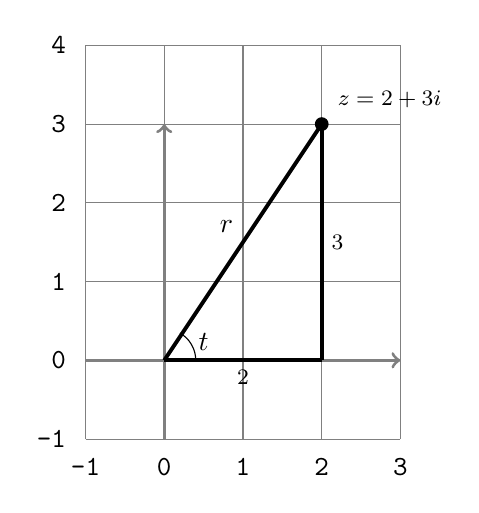
\begin{tikzpicture}
\draw[gray] (-1,-1) to  (-1,4);
\draw[gray] (0,-1) to  (0,4);
\draw[gray] (1,-1) to  (1,4);
\draw[gray] (2,-1) to  (2,4);
\draw[gray] (3,-1) to  (3,4);
\draw[gray] (-1,-1) to  (3,-1);
\draw[gray] (-1,0) to  (3,0);
\draw[gray] (-1,1) to  (3,1);
\draw[gray] (-1,2) to  (3,2);
\draw[gray] (-1,3) to  (3,3);
\draw[gray] (-1,4) to  (3,4);
\draw(-1, -1) node [font=\ttfamily, label=below:{\normalsize {\texttt{-1}}}] {};
\draw(0, -1) node [font=\ttfamily, label=below:{\normalsize {\texttt{0}}}] {};
\draw(1, -1) node [font=\ttfamily, label=below:{\normalsize {\texttt{1}}}] {};
\draw(2, -1) node [font=\ttfamily, label=below:{\normalsize {\texttt{2}}}] {};
\draw(3, -1) node [font=\ttfamily, label=below:{\normalsize {\texttt{3}}}] {};
\draw(-1, -1) node [font=\ttfamily, label=left:{\normalsize {\texttt{-1}}}] {};
\draw(-1, 0) node [font=\ttfamily, label=left:{\normalsize {\texttt{0}}}] {};
\draw(-1, 1) node [font=\ttfamily, label=left:{\normalsize {\texttt{1}}}] {};
\draw(-1, 2) node [font=\ttfamily, label=left:{\normalsize {\texttt{2}}}] {};
\draw(-1, 3) node [font=\ttfamily, label=left:{\normalsize {\texttt{3}}}] {};
\draw(-1, 4) node [font=\ttfamily, label=left:{\normalsize {\texttt{4}}}] {};
\draw[line width=0.04cm,black!50,->] (-1,0) to  (3,0);
\draw[line width=0.04cm,black!50,->] (0,-1) to  (0,3);

\fill[black] (2.0, 3.0) circle (0.08);
\draw[black] (2.0, 3.0) circle (0.08);
\node[anchor=south west] at (2.08,3.08)   {\footnotesize{$z = 2 + 3i$}};
\draw[line width=0.05cm,black] (0,0) to  (2,3);

\node[anchor=south east] at (1.0,1.5)   {$\footnotesize{r}$};
\draw[line width=0.05cm,black] (0,0) to  (2,0);

\node[anchor=north] at (1.0,0)   {\footnotesize{2}};
\draw[line width=0.05cm,black] (2,0) to  (2,3);

\node[anchor=west] at (2,1.5)   {\footnotesize{$3$}};
\draw[] (0.4,0) arc (0:60:0.4);
\node[anchor=south] at (0.5,0)   {{$t$}};
\end{tikzpicture}

\end{center}


I've added the distance of $z$ from 0, i.e. $r$ and the
angle the line from $0$ to $z$ makes with the real axis, i.e. $t$.
Again, $r$ is the distance from $z$ to $0$ and $t$ is the 
angle made by the line $\overline{0z}$ with the positive real axis.
The distance of $z$ from $0$ is written
\[
|z|
\]

OK, that great.
But we want to avoid drawing pictures because we might
not be absolutely accurate in measuring
$r$ and $t$.
By Pythagorus theorem 
\[
r = \sqrt{2^2 + 3^2} = \sqrt{13}
\]
The angle $t$ is just
\[
\tan t = \frac{3}{2}
\]
i.e.
\[
t = \tan^{-1} \frac{3}{2}
\]
In this case $t$ is approximately $0.9828$ in radians (or 56.31 degrees).
Hence
\[
z = \sqrt{13} (\cos 0.9828 + i \sin 0.9828)
\]
Hence
\[
z^n = \sqrt{13}^n (\cos 0.9828n + i \sin 0.9828n)
\]
Note that taking powers is now taking powers of a real number
(i.e. the
$\sqrt{13}$) and computing $nt$.
Of course you still need to compute sine and cosine
of the angle $nt$. 

Of course the problem is that we need to approximate angles and sines and 
cosines for the above example.
There are however standard angles that you should be aware of.
This includes $t = 0, \pi/6, \pi/4, \pi/3, \pi/2$ (corresponding to
$0, 30, 45, 60, 90$ degrees).
In these cases we can be exact.

Here's an example where you can compute the angle exactly.
Let $z = 1 + \sqrt{3} i$. In this case
\[
r = \sqrt{1 + 3} = 2
\]
and
\[
\tan t = \frac{\sqrt{3}}{1} = \sqrt{3}
\]
i.e. 
\[
t = \frac{\pi}{3}
\]
(i.e. 60 degrees).
Hence 
\[
z^n = 2^n 
\biggl( 
\cos \frac{n\pi}{3}
+ i \sin \frac{n\pi}{3}
\biggr)
\]
For instance
\[
z^{1000} = 2^{1000} 
\biggl( 
\cos \frac{1000\pi}{3}
+ i \sin \frac{1000\pi}{3}
\biggr)
\]
Now note that 
\[
\frac{1000}{3}\pi 
=
333\pi + \frac{1}{3}\pi
\]
Of course you know that the sine and cosine functions have period of $2\pi$:
\[
\frac{1000}{3}\pi 
=
166(2\pi) + \frac{4}{3} \pi
\]
Therefore
\begin{align*}
\cos \frac{1000}{3}\pi &= \cos(4\pi/3) = -1/2\\
\sin \frac{1000}{3}\pi &= \sin(4\pi/3) = -\sqrt{3}/2
\end{align*}
Therefore
\[
z^{1000} =
2^{1000}
\biggl( 
\frac{-1}{2}
+ i
\frac{-\sqrt{3}}{2}
\biggr)
\]

Let's try an example.
Derive a closed form for $a_n$ where
\begin{align*}
a_n = 
\begin{cases}
1 & \text{ if } n = 0 \\
2 & \text{ if } n = 1 \\
-a_{n-1} - a_{n-2} &\text{ if } n > 1 
\end{cases}
\end{align*}

I'll let you derive the rational function for 
$a(x) = \sum_{n=0}^\infty a_n x^n$.
It's
\[
a(x) = \frac{1 + 3x}{1 + x + x^2}
\]
The roots of $1 + x + x^2$ are (using the quadratic equation formula for roots)
\[
\frac{-1 \pm \sqrt{1 - 4}}{2}
= \frac{-1 \pm i\sqrt{3}}{2}
\]
Let 
\[
z_1 = \frac{-1 + i\sqrt{3}}{2}, \,\,\,\,\,
z_2 = \frac{-1 - i\sqrt{3}}{2}
\]

Going back to our rational function for $a(x)$ we obtain
\begin{align*}
a(x) 
&= \frac{1 + 3x}{1 + x + x^2} \\
&= \frac{1 + 3x}{(x - z_1)(x - z_2)}
\end{align*}
Of course we now need to break up the rational function into two pieces using
partial fractions.
Let
\[
\frac{1}{(x - z_1)(x - z_2)} 
= 
\frac{A}{x - z_1}
+
\frac{B}{x - z_2}
\]
therefore
\[
1 
= 
A(x - z_2)
+
B(x - z_1)
\]
Let $x = z_1$ and we get
\begin{align*}
1 
&= A(z_1 - z_2) \\
\therefore
A &= \frac{1}{z_1 - z_2}
\end{align*}
Note that


\begin{align*}
z_1 - z_2 
= \frac{-1 + i\sqrt{3}}{2} - \frac{-1 - i\sqrt{3}}{2}
= \sqrt{3}i
\end{align*}
Therefore
\begin{align*}
A 
= \frac{1}{\sqrt{3}i} \cdot \frac{-\sqrt{3}i}{-\sqrt{3}i}
= \frac{-\sqrt{3}}{3} i
\end{align*}

Now for $B$ ... if we let $x = z_2$ in 
\[
1 
= 
A(x - z_2)
+
B(x - z_1)
\]
we get
\[
1 = B(z_2 - z_1)
\]
and therefore
\[
B = \frac{1}{z_2 - z_1}
\]
If you're sharp, you'd see that $B = -A$ and therefore save you time in compute $B$ from scratch.
Therefore
\[
B = \frac{\sqrt{3}}{3} i
\]
Hence
\begin{align*}
\frac{1}{(x - z_1)(x - z_2)} 
&= \frac{A}{x - z_1} + \frac{B}{x - z_2} \\
&= \frac{-i\sqrt{3}}{3} \frac{1}{x - z_1} + \frac{i\sqrt{3}}{3} \frac{1}{x - z_2} \\
&= \frac{i\sqrt{3}}{3} \frac{1}{z_1 - x} - \frac{i\sqrt{3}}{3} \frac{1}{z_2 - x} \\
&= \frac{i\sqrt{3}}{3} \frac{1}{z_1} \frac{1}{1 - x/z_1} - \frac{i\sqrt{3}}{3} \frac{1}{z_2} \frac{1}{1 - x/z_2} \\
&= \frac{i\sqrt{3}}{3} \frac{1}{z_1} \sum_{n=0}^\infty \biggl( \frac{x}{z_1} \biggr)^n  
- \frac{i\sqrt{3}}{3} \frac{1}{z_2} \sum_{n=0}^\infty \biggl( \frac{x}{z_2} \biggr)^2 \\
&=  
\frac{i\sqrt{3}}{3}
\sum_{n=0}^\infty 
\biggl( 
\frac{1}{z_1} \biggl( \frac{1}{z_1} \biggr)^n  
-  \frac{1}{z_2} \biggl( \frac{1}{z_2} 
\biggr)^n\biggr) 
x^n\\
&=  
\frac{i\sqrt{3}}{3}
\sum_{n=0}^\infty 
\biggl( 
(z_1^{-1})^{n+1}  
-  (z_2^{-1})^{n+1} 
\biggr) 
x^n
\end{align*}

Uh-oh ... now we need to compute powers of $z_1$ and $z_2$.
We can use binomial theorem ... but we're going to use de Moivre's theorem instead.
If I draw $z_1$ and $z_2$ on the complex plane I get
\begin{center}
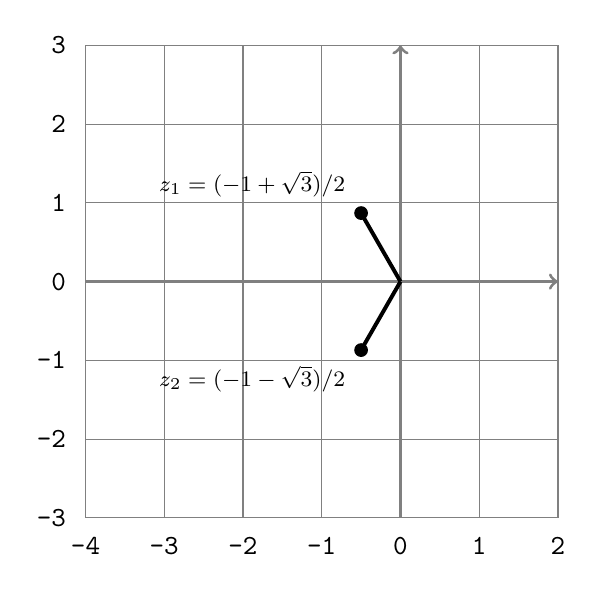
\begin{tikzpicture}
\draw[gray] (-4,-3) to  (-4,3);
\draw[gray] (-3,-3) to  (-3,3);
\draw[gray] (-2,-3) to  (-2,3);
\draw[gray] (-1,-3) to  (-1,3);
\draw[gray] (0,-3) to  (0,3);
\draw[gray] (1,-3) to  (1,3);
\draw[gray] (2,-3) to  (2,3);
\draw[gray] (-4,-3) to  (2,-3);
\draw[gray] (-4,-2) to  (2,-2);
\draw[gray] (-4,-1) to  (2,-1);
\draw[gray] (-4,0) to  (2,0);
\draw[gray] (-4,1) to  (2,1);
\draw[gray] (-4,2) to  (2,2);
\draw[gray] (-4,3) to  (2,3);
\draw(-4, -3) node [font=\ttfamily, label=below:{\normalsize {\texttt{-4}}}] {};
\draw(-3, -3) node [font=\ttfamily, label=below:{\normalsize {\texttt{-3}}}] {};
\draw(-2, -3) node [font=\ttfamily, label=below:{\normalsize {\texttt{-2}}}] {};
\draw(-1, -3) node [font=\ttfamily, label=below:{\normalsize {\texttt{-1}}}] {};
\draw(0, -3) node [font=\ttfamily, label=below:{\normalsize {\texttt{0}}}] {};
\draw(1, -3) node [font=\ttfamily, label=below:{\normalsize {\texttt{1}}}] {};
\draw(2, -3) node [font=\ttfamily, label=below:{\normalsize {\texttt{2}}}] {};
\draw(-4, -3) node [font=\ttfamily, label=left:{\normalsize {\texttt{-3}}}] {};
\draw(-4, -2) node [font=\ttfamily, label=left:{\normalsize {\texttt{-2}}}] {};
\draw(-4, -1) node [font=\ttfamily, label=left:{\normalsize {\texttt{-1}}}] {};
\draw(-4, 0) node [font=\ttfamily, label=left:{\normalsize {\texttt{0}}}] {};
\draw(-4, 1) node [font=\ttfamily, label=left:{\normalsize {\texttt{1}}}] {};
\draw(-4, 2) node [font=\ttfamily, label=left:{\normalsize {\texttt{2}}}] {};
\draw(-4, 3) node [font=\ttfamily, label=left:{\normalsize {\texttt{3}}}] {};
\draw[line width=0.04cm,black!50,->] (-4,0) to  (2,0);
\draw[line width=0.04cm,black!50,->] (0,-3) to  (0,3);

\fill[black] (-0.5, 0.87) circle (0.08);
\draw[black] (-0.5, 0.87) circle (0.08);
\node[anchor=south east] at (-0.58,0.946)   {\footnotesize{$z_1 = (-1+\sqrt{3})/2$}};
\draw[line width=0.05cm,black] (0,0) to  (-0.5,0.87);

\fill[black] (-0.5, -0.87) circle (0.08);
\draw[black] (-0.5, -0.87) circle (0.08);
\node[anchor=north east] at (-0.58,-0.946)   {\footnotesize{$z_2 = (-1-\sqrt{3})/2$}};
\draw[line width=0.05cm,black] (0,0) to  (-0.5,-0.87);
\end{tikzpicture}

\end{center}


Let's focus on $z_1$.
The distance of $z_1$ from $0$, let's call it $r_1$ is
\[
|z_1| = r_1 = \sqrt{ \biggl( \frac{\sqrt{3}}{2} \biggr)^2 + \biggl( \frac{-1}{2} \biggr)^2 } = 1
\]

%-*-latex-*-

\begin{ex} 
  \label{ex:prob-00}
  \tinysidebar{\debug{exercises/{disc-prob-28/question.tex}}}

  \solutionlink{sol:prob-00}
  \qed
\end{ex} 
\begin{python0}
from solutions import *
add(label="ex:prob-00",
    srcfilename='exercises/discrete-probability/prob-00/answer.tex') 
\end{python0}


Now for the angle.
\begin{center}
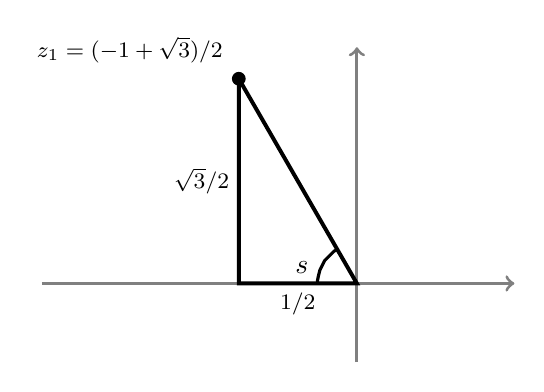
\begin{tikzpicture}
\draw[line width=0.04cm,black!50,->] (-4,0) to  (2,0);
\draw[line width=0.04cm,black!50,->] (0,-1) to  (0,3);

\fill[black] (-1.5, 2.6) circle (0.08);
\draw[black] (-1.5, 2.6) circle (0.08);
\node[anchor=south east] at (-1.58,2.678)   {\footnotesize{$z_1 = (-1+\sqrt{3})/2$}};
\draw[line width=0.04cm,black] (-0.25,0.43) to  (-0.29,0.41) to  (-0.32,0.38) to  (-0.35,0.35) to  (-0.38,0.32) to  (-0.41,0.29) to  (-0.43,0.25) to  (-0.45,0.21) to  (-0.47,0.17) to  (-0.48,0.13) to  (-0.49,0.09) to  (-0.5,0.04) to  (-0.5,0.0) to  (-0.5,0.0);

\node[anchor=south] at (-0.7,0)   {{$s$}};
\draw[line width=0.05cm,black] (-1.5,2.6) to  (-1.5,0) to  (0,0) to  (-1.5,2.6);

\node[anchor=north] at (-0.75,0)   {\footnotesize{1/2}};

\node[anchor=east] at (-1.5,1.299)   {\footnotesize{$\sqrt{3}/2$}};
\end{tikzpicture}

\end{center}


Angle $s$ satisfies
\[
\tan s = \frac{\sqrt{3}/2}{1/2} = \sqrt{3}
\]
This is one of the standard angles: $s = \pi/3$ (i.e. 60 degrees).
However remember that the angle we want is the angle that $z_1$ makes with 
the positive real axis:
\begin{center}
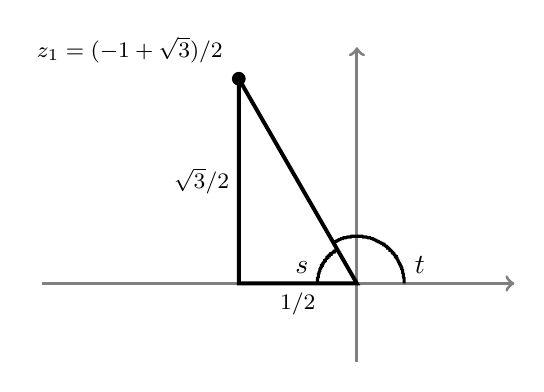
\begin{tikzpicture}
\draw[line width=0.04cm,black!50,->] (-4,0) to  (2,0);
\draw[line width=0.04cm,black!50,->] (0,-1) to  (0,3);

\fill[black] (-1.5, 2.6) circle (0.08);
\draw[black] (-1.5, 2.6) circle (0.08);
\node[anchor=south east] at (-1.58,2.678)   {\footnotesize{$z_1 = (-1+\sqrt{3})/2$}};
\draw[line width=0.04cm,black] (-0.25,0.43) to  (-0.26,0.43) to  (-0.27,0.42) to  (-0.27,0.42) to  (-0.28,0.41) to  (-0.29,0.41) to  (-0.29,0.4) to  (-0.3,0.4) to  (-0.31,0.39) to  (-0.31,0.39) to  (-0.32,0.38) to  (-0.33,0.38) to  (-0.33,0.37) to  (-0.34,0.37) to  (-0.35,0.36) to  (-0.35,0.35) to  (-0.36,0.35) to  (-0.37,0.34) to  (-0.37,0.33) to  (-0.38,0.33) to  (-0.38,0.32) to  (-0.39,0.31) to  (-0.39,0.31) to  (-0.4,0.3) to  (-0.4,0.29) to  (-0.41,0.29) to  (-0.41,0.28) to  (-0.42,0.27) to  (-0.42,0.27) to  (-0.43,0.26) to  (-0.43,0.25) to  (-0.44,0.24) to  (-0.44,0.23) to  (-0.45,0.23) to  (-0.45,0.22) to  (-0.45,0.21) to  (-0.46,0.2) to  (-0.46,0.2) to  (-0.46,0.19) to  (-0.47,0.18) to  (-0.47,0.17) to  (-0.47,0.16) to  (-0.48,0.15) to  (-0.48,0.15) to  (-0.48,0.14) to  (-0.48,0.13) to  (-0.49,0.12) to  (-0.49,0.11) to  (-0.49,0.1) to  (-0.49,0.1) to  (-0.49,0.09) to  (-0.49,0.08) to  (-0.5,0.07) to  (-0.5,0.06) to  (-0.5,0.05) to  (-0.5,0.04) to  (-0.5,0.03) to  (-0.5,0.03) to  (-0.5,0.02) to  (-0.5,0.01) to  (-0.5,0.0);

\node[anchor=south] at (-0.7,0)   {{$s$}};
\draw[line width=0.04cm,black] (0.6,0.0) to  (0.6,0.01) to  (0.6,0.02) to  (0.6,0.03) to  (0.6,0.04) to  (0.6,0.05) to  (0.6,0.06) to  (0.6,0.07) to  (0.59,0.08) to  (0.59,0.09) to  (0.59,0.1) to  (0.59,0.11) to  (0.59,0.12) to  (0.58,0.14) to  (0.58,0.15) to  (0.58,0.16) to  (0.58,0.17) to  (0.57,0.18) to  (0.57,0.19) to  (0.57,0.2) to  (0.56,0.21) to  (0.56,0.21) to  (0.56,0.22) to  (0.55,0.23) to  (0.55,0.24) to  (0.54,0.25) to  (0.54,0.26) to  (0.53,0.27) to  (0.53,0.28) to  (0.52,0.29) to  (0.52,0.3) to  (0.51,0.31) to  (0.51,0.32) to  (0.5,0.33) to  (0.5,0.34) to  (0.49,0.34) to  (0.49,0.35) to  (0.48,0.36) to  (0.47,0.37) to  (0.47,0.38) to  (0.46,0.39) to  (0.45,0.39) to  (0.45,0.4) to  (0.44,0.41) to  (0.43,0.42) to  (0.42,0.42) to  (0.42,0.43) to  (0.41,0.44) to  (0.4,0.45) to  (0.39,0.45) to  (0.39,0.46) to  (0.38,0.47) to  (0.37,0.47) to  (0.36,0.48) to  (0.35,0.49) to  (0.34,0.49) to  (0.34,0.5) to  (0.33,0.5) to  (0.32,0.51) to  (0.31,0.51) to  (0.3,0.52) to  (0.29,0.52) to  (0.28,0.53) to  (0.27,0.53) to  (0.26,0.54) to  (0.25,0.54) to  (0.24,0.55) to  (0.23,0.55) to  (0.22,0.56) to  (0.21,0.56) to  (0.21,0.56) to  (0.2,0.57) to  (0.19,0.57) to  (0.18,0.57) to  (0.17,0.58) to  (0.16,0.58) to  (0.15,0.58) to  (0.14,0.58) to  (0.12,0.59) to  (0.11,0.59) to  (0.1,0.59) to  (0.09,0.59) to  (0.08,0.59) to  (0.07,0.6) to  (0.06,0.6) to  (0.05,0.6) to  (0.04,0.6) to  (0.03,0.6) to  (0.02,0.6) to  (0.01,0.6) to  (0.0,0.6) to  (-0.01,0.6) to  (-0.02,0.6) to  (-0.03,0.6) to  (-0.04,0.6) to  (-0.05,0.6) to  (-0.06,0.6) to  (-0.07,0.6) to  (-0.08,0.59) to  (-0.09,0.59) to  (-0.1,0.59) to  (-0.11,0.59) to  (-0.12,0.59) to  (-0.14,0.58) to  (-0.15,0.58) to  (-0.16,0.58) to  (-0.17,0.58) to  (-0.18,0.57) to  (-0.19,0.57) to  (-0.2,0.57) to  (-0.21,0.56) to  (-0.21,0.56) to  (-0.22,0.56) to  (-0.23,0.55) to  (-0.24,0.55) to  (-0.25,0.54) to  (-0.26,0.54) to  (-0.27,0.53) to  (-0.28,0.53) to  (-0.29,0.52) to  (-0.3,0.52);

\node[anchor=south] at (0.8,0)   {{$t$}};
\draw[line width=0.05cm,black] (-1.5,2.6) to  (-1.5,0) to  (0,0) to  (-1.5,2.6);

\node[anchor=north] at (-0.75,0)   {\footnotesize{1/2}};

\node[anchor=east] at (-1.5,1.299)   {\footnotesize{$\sqrt{3}/2$}};
\end{tikzpicture}

\end{center}


We have
\[
t = \pi - s = \frac{2\pi}{3}
\]

Therefore $z_1$ in polar coordinates is $1 (\cos (2\pi/3) + i \sin(2\pi/3))$, i.e.
\[
z_1 = -\frac{1}{2} + \frac{\sqrt{3}}{2}i = \cos \biggl( \frac{2\pi}{3} \biggr) + i \sin \biggl( \frac{2\pi}{3} \biggl)
\]

I'll leave it to you to show
\[
z_2 = \cos \biggl( -\frac{2\pi}{3} \biggr) + i \sin \biggl( -\frac{2\pi}{3} \biggl)
\]

Let's collect all the facts together just to know where we are.
First we have the rational function of our generating function:
\[
a(x) = \frac{1 + 3x}{1 + x + x^2}
\]
The denominator is rewritten as
\begin{align*}
\frac{1}{1 + x + x^2}
&=
\frac{i\sqrt{3}}{3}
\sum_{n=0}^\infty 
\biggl( 
(z_1^{-1})^{n+1}  
-  (z_2^{-1})^{n+1} 
\biggr) 
x^n
\end{align*}
where
\[
z_1 = -\frac{1}{2} + \frac{\sqrt{3}}{2}i = \cos \biggl( \frac{2\pi}{3} \biggr) + i \sin \biggl( \frac{2\pi}{3} \biggl)
\]
and
\[
z_2 = -\frac{1}{2} + \frac{\sqrt{3}}{2}i = \cos \biggl( -\frac{2\pi}{3} \biggr) + i \sin \biggl( -\frac{2\pi}{3} \biggl)
\]

Now
\begin{align*}
z_1^{-1} 
&= \frac{1}{\cos \bigl( \frac{2\pi}{3} \bigr) + i \sin \bigl( \frac{2\pi}{3} \bigl)}
\cdot \frac{\cos \bigl( \frac{2\pi}{3} \bigr) - i \sin \bigl( \frac{2\pi}{3} \bigl)}{\cos \bigl( \frac{2\pi}{3} \bigr) - i \sin \bigl( \frac{2\pi}{3} \bigl)} \\
&= \frac{\cos \bigl( \frac{2\pi}{3} \bigr) - i \sin \bigl( \frac{2\pi}{3} \bigl)}{1} \\
&= z_2
\end{align*}
and therefore $z_2^{-1} = z_1$.
Hence
\begin{align*}
\frac{1}{1 + x + x^2}
&=
\frac{i\sqrt{3}}{3}
\sum_{n=0}^\infty 
\biggl( 
(z_1^{-1})^{n+1}  
-  (z_2^{-1})^{n+1} 
\biggr) 
x^n \\
&=
\frac{i\sqrt{3}}{3}
\sum_{n=0}^\infty 
\biggl( 
z_2^{n+1}  
-  z_1^{n+1} 
\biggr) 
x^n
\end{align*}
By de Moivre's theorem,
\[
z_1^{n+1} = \cos \biggl( \frac{2(n+1)\pi}{3} \biggr) + i \sin \biggl( \frac{2(n+1)\pi}{3} \biggl)
\]
and
\begin{align*}
z_2^{n+1} 
&= \cos \biggl( -\frac{2(n+1)\pi}{3} \biggr) + i \sin \biggl( -\frac{2(n+1)\pi}{3} \biggl) \\
&= \cos \biggl( \frac{2(n+1)\pi}{3} \biggr) - i \sin \biggl( \frac{2(n+1)\pi}{3} \biggl) \\
\end{align*}
Together we have
\begin{align*}
z_2^{n+1} - z_1^{n+1}
&= \cos \biggl( \frac{2(n+1)\pi}{3} \biggr) - i \sin \biggl( \frac{2(n+1)\pi}{3} \biggl) \\
&\hskip 0.5cm -\cos \biggl( \frac{2(n+1)\pi}{3} \biggr) - i \sin \biggl( \frac{2(n+1)\pi}{3} \biggl) \\
&= -2i \sin \frac{2(n+1)\pi}{3}
\end{align*}
Hence our rational $\displaystyle \frac{1}{1+x+x^2}$ becomes
\begin{align*}
\frac{1}{1 + x + x^2}
&= 
\frac{i\sqrt{3}}{3} 
\sum_{n=0}^\infty 
\biggl( -2i \sin \frac{2(n+1)\pi}{3} \biggr) x^n \\
&= 
\frac{2\sqrt{3}}{3} 
\sum_{n=0}^\infty
\biggl( \sin \frac{2(n+1)\pi}{3} \biggr)
x^n \\
\end{align*}

I want to consider cases for $n = 3m, 3m+1, 3m+2$ (... why? to kill the 
denominator 3 of course!)
Let $n = 3m + k$. 
Then 
\begin{align*}
\sin \frac{2(3m+k+1)\pi}{3}
&= \sin \biggl( 2m\pi  + \frac{2(k+1)}{3} \pi \biggr) \\
&= \sin \biggl( \frac{2(k+1)}{3} \pi \biggr) \\
&=
\begin{cases}
\sin \bigl( \frac{2}{3} \pi \bigr) &\text{ if } k = 0 \\
\sin \bigl( \frac{4}{3} \pi \bigr) &\text{ if } k = 1 \\
\sin \bigl( \frac{6}{3} \pi \bigr) &\text{ if } k = 2 \\
\end{cases} \\
&=
\begin{cases}
\sin \bigl( \frac{1}{3} \pi \bigr) &\text{ if } k = 0 \\
-\sin \bigl( \frac{1}{3} \pi \bigr) &\text{ if } k = 1 \\
0 &\text{ if } k = 2 \\
\end{cases} \\
&=
\begin{cases}
\frac{\sqrt{3}}{2} &\text{ if } k = 0 \\
-\frac{\sqrt{3}}{2} &\text{ if } k = 1 \\
0 &\text{ if } k = 2 \\
\end{cases}
\end{align*}
Therefore
\begin{align*}
\frac{2\sqrt{3}}{3} \sin \frac{2(n+1)\pi}{3}
&= 
\begin{cases}
\frac{2\sqrt{3}}{3} \cdot \frac{\sqrt{3}}{2} &\text{ if } n = 3m \\
-\frac{2\sqrt{3}}{3} \cdot \frac{\sqrt{3}}{2} &\text{ if } n = 3m+1 \\
0 &\text{ if } n = 3m+2 \\
\end{cases} \\
&= 
\begin{cases}
1 &\text{ if } n = 3m \\
-1 &\text{ if } n = 3m+1 \\
0 &\text{ if } n = 3m+2 \\
\end{cases}
\end{align*}
Recall that
\begin{align*}
\frac{1}{1 + x + x^2}
&= 
\sum_{n=0}^\infty
\frac{2\sqrt{3}}{3} 
\biggl( \sin \frac{2(n+1)\pi}{3} \biggr)
x^n \\
\end{align*}
Instead of trying to force the series to contain all three cases,
I'll write it as 3 separate series:
\begin{align*}
\frac{1}{1 + x + x^2}
&= 
\sum_{m=0}^\infty x^{3m} +
\sum_{m=0}^\infty (-1)x^{3m+1}
\sum_{m=0}^\infty 0x^{3m+2} \\
&= 
\sum_{m=0}^\infty x^{3m} +
\sum_{m=0}^\infty (-1)x^{3m+1}
\end{align*}

At this point it's a good idea to check the computations numerically with 
a program:
\begin{Verbatim}[frame=single,fontsize=\footnotesize]
>>> def f(x): return 1.0/(1+x+x*x)
...
>>> def g(x):
...     s = 0.0
...     for n in range(1000000):
...         import math
...         if n % 3 == 0: s += x**n
...         elif n % 3 == 1: s += -x**n
...     return s
...
>>> f(0.5)
0.5714285714285714
>>> g(0.5)
0.5714285714285714
>>> f(0.25)
0.76190476190476186
>>> g(0.25)
0.76190476190476186
>>>
\end{Verbatim}
Good! Onward!

And now (finally), 
\begin{align*}
a(x) 
&= (1 + 3x) \cdot \frac{1}{1 + x + x^2} \\
&= 
(1 + 3x) 
\biggl( 
\sum_{m=0}^\infty x^{3m} +
\sum_{m=0}^\infty (-1)x^{3m+1}\biggr) \\
&=  
\sum_{m=0}^\infty x^{3m} +
\sum_{m=0}^\infty (-1)x^{3m+1}  \\
&\hskip 1cm + 3x
\biggl( 
\sum_{m=0}^\infty x^{3m} +
\sum_{m=0}^\infty (-1)x^{3m+1}\biggr) \\
&=   
\sum_{m=0}^\infty x^{3m} +
\sum_{m=0}^\infty (-1)x^{3m+1}  \\
&\hskip 1cm +
\sum_{m=0}^\infty 3x^{3m+1} +
\sum_{m=0}^\infty (-3)x^{3m+2} \\
&=   
\sum_{m=0}^\infty x^{3m} +
\sum_{m=0}^\infty 2x^{3m+1}
\sum_{m=0}^\infty (-3)x^{3m+2} \\
\end{align*}
i.e.
\[
a_n = 
\begin{cases}
1  &\text{ if } n = 3m \\
2  &\text{ if } n = 3m + 1\\
-3 &\text{ if } n = 3m + 2\\
\end{cases}
\]

Whoa!!! Can it be that simple?!?
Let's check it with the definition of our $a_n$ via recurrences
\begin{align*}
a_n = 
\begin{cases}
1 & \text{ if } n = 0 \\
2 & \text{ if } n = 1 \\
-a_{n-1} - a_{n-2} &\text{ if } n > 1 
\end{cases}
\end{align*}

Well ... \textit{is} true for $a_0$, $a_1$.
What about the rest?
\begin{align*}
a_2 &= -a_1 - a_0 = -2-1 = -3 \\
a_3 &= -a_2 -a_1 = -(-3) - 1 = 2 \\
a_4 &= -a_3-a_2 = -2+3 = 1 \\
a_5 &= -a_4-a_3 = -1-2 = -3 \\
a_6 &= -a_5-a_4 = -(-3)-1 = 2 \\
a_7 &= -a_6-a_5 = -2-(-3) = 1 \\
a_8 &= -a_7-a_6 = -1-2 = -3 \\
a_9 &= -a_8-a_7 = -(-3)-1 = -2 \\
\end{align*}
and now note that the last two lines of checks begin to repeat earlier ones.

Neat right?
\vfill\eject
